\section{Auswertung}
\subsection{Aufnahme der Hysterese}
Die gemessenen magnetischen Flussdichten $B$ in Abhängigkeit der angelegten Stromstärke $I$
sind in Tabelle \ref{tab: hysterese} aufgetragen. Eine graphische Darstellung befindet sich in Abbildung
\ref{fig: hysterese_gesamt}. Mittels der Messwerte wird eine Regression nach dem Prinzip der kleinsten Quadrate
an eine Funktion der Form
\begin{equation}
  B(I) = a_1 I^3 + a_2 I^2 + a_3 I ^2 + a_4
  \label{eq: fitfuntion_hysterese}
\end{equation}
bestimmt. Für den austeigenden Ast der Hysterese ergeben sich folgende Parameter
\begin{align}
  \begin{aligned}
    a_1 &= \SI{-0.7(1)e-1}{\milli\tesla \per \ampere ^3} & a_2 &= \SI{1.5(3)}{\milli\tesla \per \ampere ^2} \\
    a_3 &= \SI{5.1(3)e1}{\milli\tesla \per \ampere } & a_4 &= \SI{3(6)}{\milli\tesla }.
    \label{eq: params_up}
  \end{aligned}
\end{align}
Analog werden folgende Werte für den absteigenden Ast gefunden
\begin{align}
  \begin{aligned}
    b_1 &= \SI{-8.6(8)e-2}{\milli\tesla \per \ampere ^3} & b_2 &= \SI{1.9(3)}{\milli\tesla \per \ampere ^2} \\
    b_3 &= \SI{4.7(2)e1}{\milli\tesla \per \ampere } & b_4 &= \SI{11(4)}{\milli\tesla }.
  \end{aligned}
\end{align}
Eine graphische Darstellung der Fitfunktionen befindet sich in Abbildung \ref{fig: hysterese_fit}.
\subsection{Aufnahme der Hysterese}
Die gemessenen magnetischen Flussdichten $B$ in Abhängigkeit der angelegten Stromstärke $I$
sind in Tabelle \ref{tab: hysterese} aufgetragen. Eine graphische Darstellung befindet sich in Abbildung
\ref{fig: hysterese_gesamt}. Mittels der Messwerte wird eine Regression nach dem Prinzip der kleinsten Quadrate
an eine Funktion der Form
\begin{equation}
  B(I) = a_1 I^3 + a_2 I^2 + a_3 I ^2 + a_4
  \label{eq: fitfuntion_hysterese}
\end{equation}
bestimmt. Für den austeigenden Ast der Hysterese ergeben sich folgende Parameter
\begin{align}
  \begin{aligned}
    a_1 &= \SI{-0.7(1)e-1}{\milli\tesla \per \ampere ^3} & a_2 &= \SI{1.5(3)}{\milli\tesla \per \ampere ^2} \\
    a_3 &= \SI{5.1(3)e1}{\milli\tesla \per \ampere } & a_4 &= \SI{3(6)}{\milli\tesla }.
    \label{eq: params_up}
  \end{aligned}
\end{align}
Analog werden folgende Werte für den absteigenden Ast gefunden
\begin{align}
  \begin{aligned}
    b_1 &= \SI{-8.6(8)e-2}{\milli\tesla \per \ampere ^3} & b_2 &= \SI{1.9(3)}{\milli\tesla \per \ampere ^2} \\
    b_3 &= \SI{4.7(2)e1}{\milli\tesla \per \ampere } & b_4 &= \SI{11(4)}{\milli\tesla }.
  \end{aligned}
\end{align}
Eine graphische Darstellung der Fitfunktionen befindet sich in Abbildung \ref{fig: hysterese_fit}.
\subsection{Aufnahme der Hysterese}
Die gemessenen magnetischen Flussdichten $B$ in Abhängigkeit der angelegten Stromstärke $I$
sind in Tabelle \ref{tab: hysterese} aufgetragen. Eine graphische Darstellung befindet sich in Abbildung
\ref{fig: hysterese_gesamt}. Mittels der Messwerte wird eine Regression nach dem Prinzip der kleinsten Quadrate
an eine Funktion der Form
\begin{equation}
  B(I) = a_1 I^3 + a_2 I^2 + a_3 I ^2 + a_4
  \label{eq: fitfuntion_hysterese}
\end{equation}
bestimmt. Für den austeigenden Ast der Hysterese ergeben sich folgende Parameter
\begin{align}
  \begin{aligned}
    a_1 &= \SI{-0.7(1)e-1}{\milli\tesla \per \ampere ^3} & a_2 &= \SI{1.5(3)}{\milli\tesla \per \ampere ^2} \\
    a_3 &= \SI{5.1(3)e1}{\milli\tesla \per \ampere } & a_4 &= \SI{3(6)}{\milli\tesla }.
    \label{eq: params_up}
  \end{aligned}
\end{align}
Analog werden folgende Werte für den absteigenden Ast gefunden
\begin{align}
  \begin{aligned}
    b_1 &= \SI{-8.6(8)e-2}{\milli\tesla \per \ampere ^3} & b_2 &= \SI{1.9(3)}{\milli\tesla \per \ampere ^2} \\
    b_3 &= \SI{4.7(2)e1}{\milli\tesla \per \ampere } & b_4 &= \SI{11(4)}{\milli\tesla }.
  \end{aligned}
\end{align}
Eine graphische Darstellung der Fitfunktionen befindet sich in Abbildung \ref{fig: hysterese_fit}.
\subsection{Aufnahme der Hysterese}
Die gemessenen magnetischen Flussdichten $B$ in Abhängigkeit der angelegten Stromstärke $I$
sind in Tabelle \ref{tab: hysterese} aufgetragen. Eine graphische Darstellung befindet sich in Abbildung
\ref{fig: hysterese_gesamt}. Mittels der Messwerte wird eine Regression nach dem Prinzip der kleinsten Quadrate
an eine Funktion der Form
\begin{equation}
  B(I) = a_1 I^3 + a_2 I^2 + a_3 I ^2 + a_4
  \label{eq: fitfuntion_hysterese}
\end{equation}
bestimmt. Für den austeigenden Ast der Hysterese ergeben sich folgende Parameter
\begin{align}
  \begin{aligned}
    a_1 &= \SI{-0.7(1)e-1}{\milli\tesla \per \ampere ^3} & a_2 &= \SI{1.5(3)}{\milli\tesla \per \ampere ^2} \\
    a_3 &= \SI{5.1(3)e1}{\milli\tesla \per \ampere } & a_4 &= \SI{3(6)}{\milli\tesla }.
    \label{eq: params_up}
  \end{aligned}
\end{align}
Analog werden folgende Werte für den absteigenden Ast gefunden
\begin{align}
  \begin{aligned}
    b_1 &= \SI{-8.6(8)e-2}{\milli\tesla \per \ampere ^3} & b_2 &= \SI{1.9(3)}{\milli\tesla \per \ampere ^2} \\
    b_3 &= \SI{4.7(2)e1}{\milli\tesla \per \ampere } & b_4 &= \SI{11(4)}{\milli\tesla }.
  \end{aligned}
\end{align}
Eine graphische Darstellung der Fitfunktionen befindet sich in Abbildung \ref{fig: hysterese_fit}.
\input{../Messdaten/tabs/hysterese.tex}
\begin{figure}
  \centering
  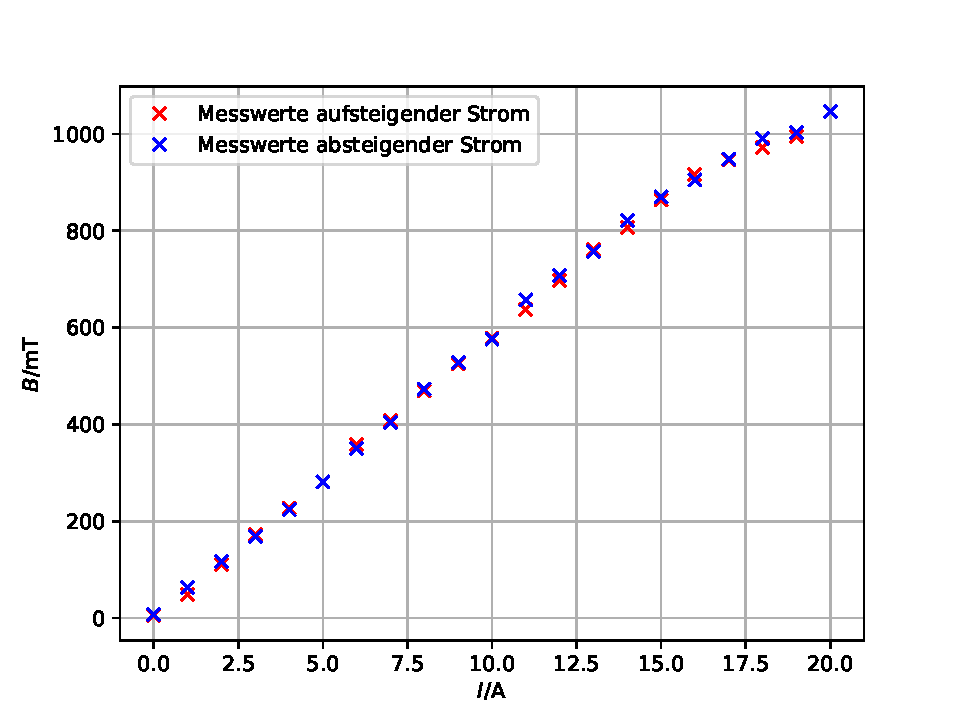
\includegraphics[width = \textwidth]{../Messdaten/plots/hysterese_data.pdf}
  \caption{Graphische Darstellung der Messwerte zur Bestimmung des Zusammenhangs $B(I)$ zwischen angelegtem Strom $I$ und
  magnetischer Flussdichte $B$ des Elektromagneten.}
  \label{fig: hysterese_gesamt}
\end{figure}
\begin{figure}
  \centering
  \begin{subfigure}{0.48\textwidth}
    \centering
  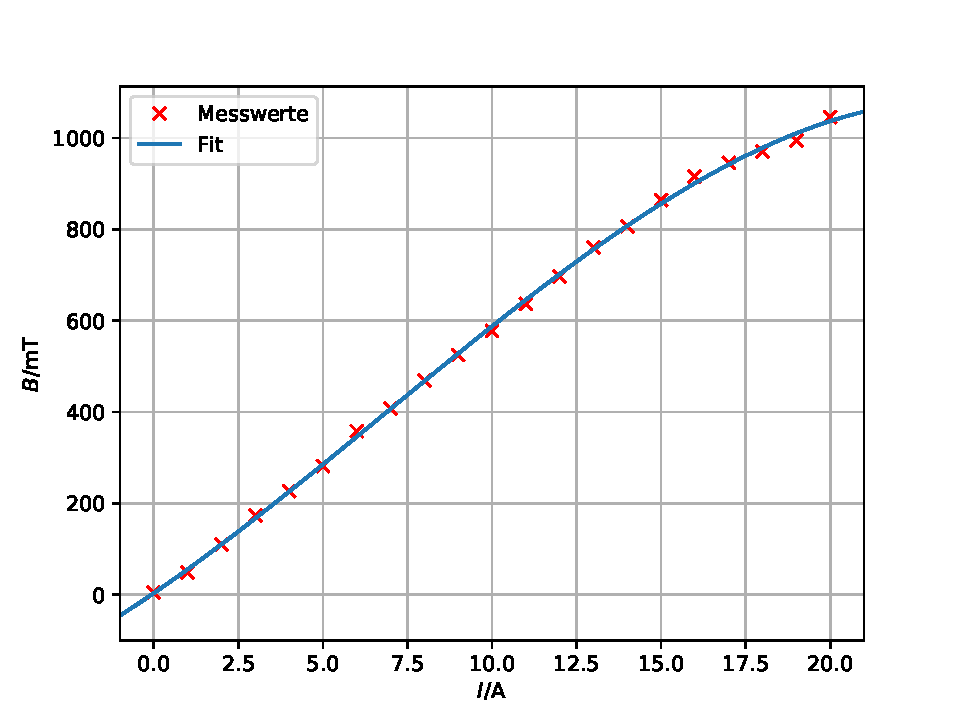
\includegraphics[width = \textwidth]{../Messdaten/plots/hysterese_aufsteigend.pdf}
  \caption{Aufsteigender Strom $I$.}
  \label{fig: hysterese_aufsteigend}
\end{subfigure}
\hfill
  \begin{subfigure}{0.48\textwidth}
  \centering
  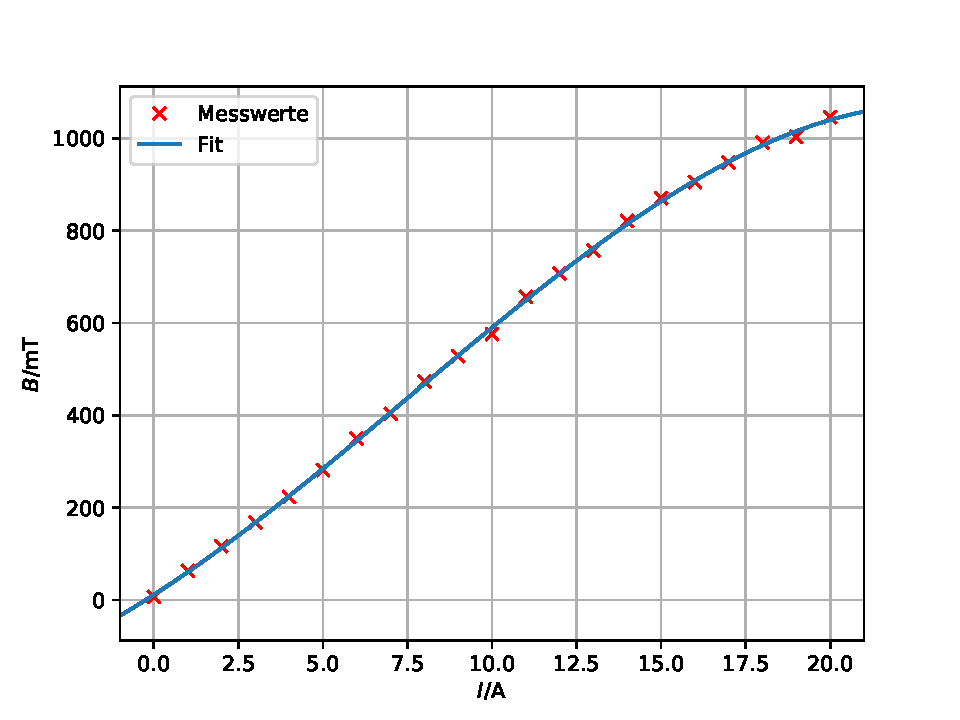
\includegraphics[width = \textwidth]{../Messdaten/plots/hysterese_absteigend.pdf}
  \caption{Absteigender Strom $I$.}
  \label{fig: hysterese_absteigend}
\end{subfigure}
\caption{Graphische Darstellung der Abhängigkeit $B(I)$ unter ab-/aufsteigendem Strom $I$ mit jeweiliger Regressionskurve.}
\label{fig: hysterese_fit}
\end{figure}
Im Folgenden wird Gleichung \eqref{eq: fitfuntion_hysterese} mit den Parametern \eqref{eq: params_up}
verwendet um den notwendigen Zusammenhang zwischen angelegtem Strom $I$ und magnetischer Flussdichte $B$ herzustellen.

\begin{figure}
  \centering
  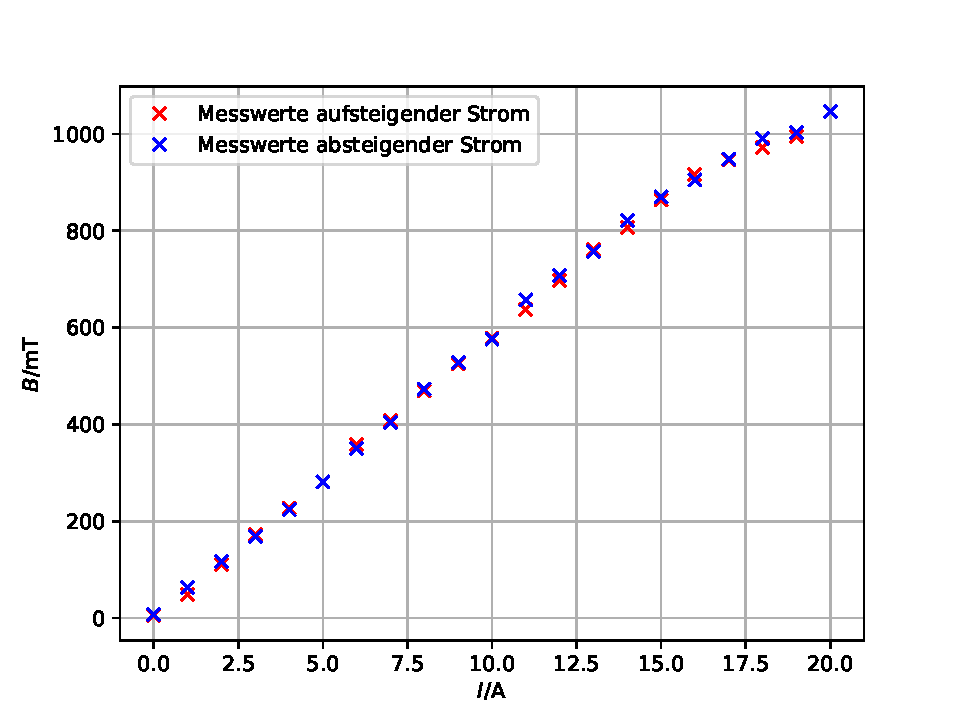
\includegraphics[width = \textwidth]{../Messdaten/plots/hysterese_data.pdf}
  \caption{Graphische Darstellung der Messwerte zur Bestimmung des Zusammenhangs $B(I)$ zwischen angelegtem Strom $I$ und
  magnetischer Flussdichte $B$ des Elektromagneten.}
  \label{fig: hysterese_gesamt}
\end{figure}
\begin{figure}
  \centering
  \begin{subfigure}{0.48\textwidth}
    \centering
  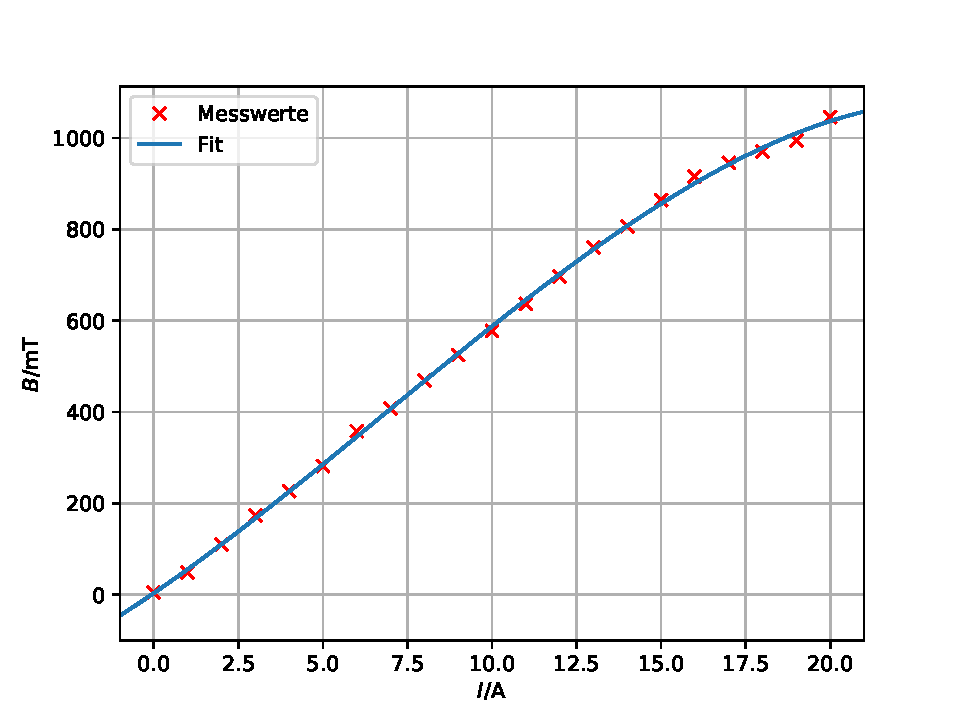
\includegraphics[width = \textwidth]{../Messdaten/plots/hysterese_aufsteigend.pdf}
  \caption{Aufsteigender Strom $I$.}
  \label{fig: hysterese_aufsteigend}
\end{subfigure}
\hfill
  \begin{subfigure}{0.48\textwidth}
  \centering
  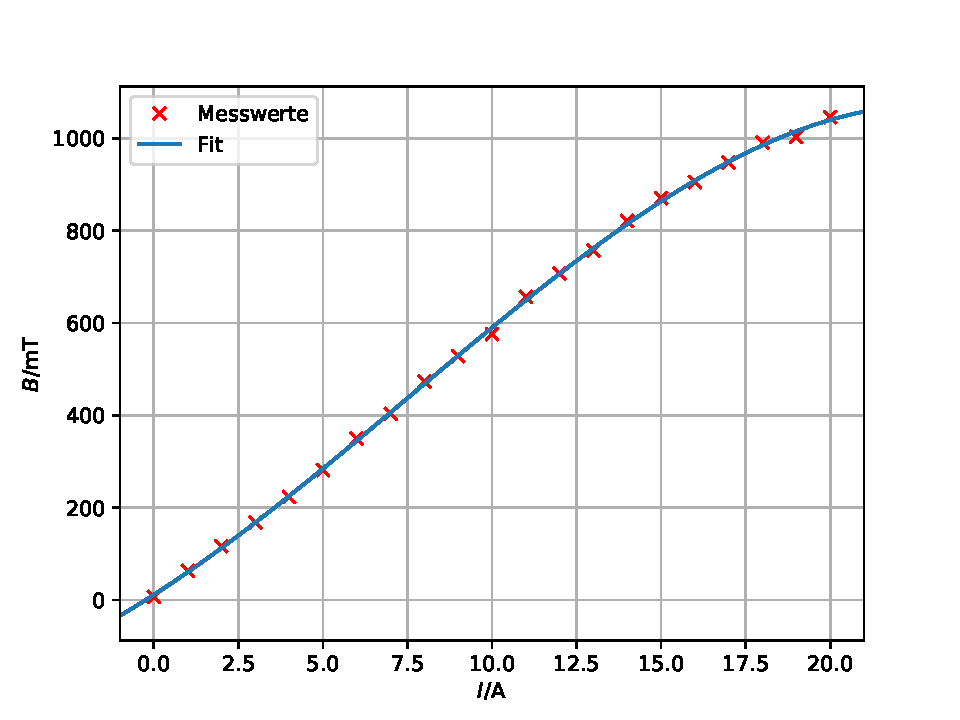
\includegraphics[width = \textwidth]{../Messdaten/plots/hysterese_absteigend.pdf}
  \caption{Absteigender Strom $I$.}
  \label{fig: hysterese_absteigend}
\end{subfigure}
\caption{Graphische Darstellung der Abhängigkeit $B(I)$ unter ab-/aufsteigendem Strom $I$ mit jeweiliger Regressionskurve.}
\label{fig: hysterese_fit}
\end{figure}
Im Folgenden wird Gleichung \eqref{eq: fitfuntion_hysterese} mit den Parametern \eqref{eq: params_up}
verwendet um den notwendigen Zusammenhang zwischen angelegtem Strom $I$ und magnetischer Flussdichte $B$ herzustellen.

\begin{figure}
  \centering
  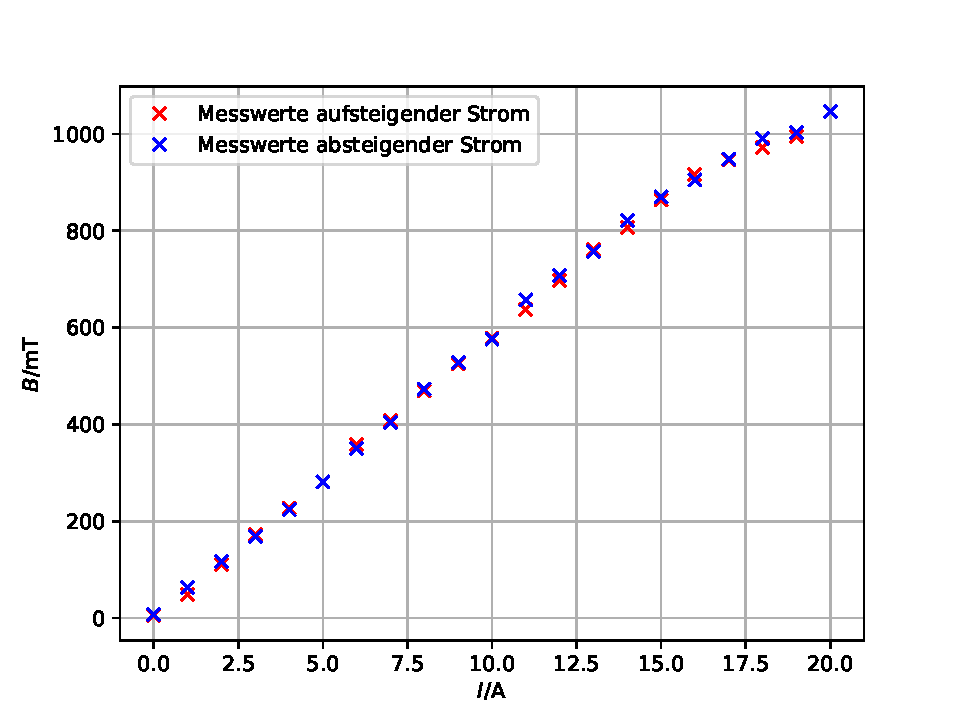
\includegraphics[width = \textwidth]{../Messdaten/plots/hysterese_data.pdf}
  \caption{Graphische Darstellung der Messwerte zur Bestimmung des Zusammenhangs $B(I)$ zwischen angelegtem Strom $I$ und
  magnetischer Flussdichte $B$ des Elektromagneten.}
  \label{fig: hysterese_gesamt}
\end{figure}
\begin{figure}
  \centering
  \begin{subfigure}{0.48\textwidth}
    \centering
  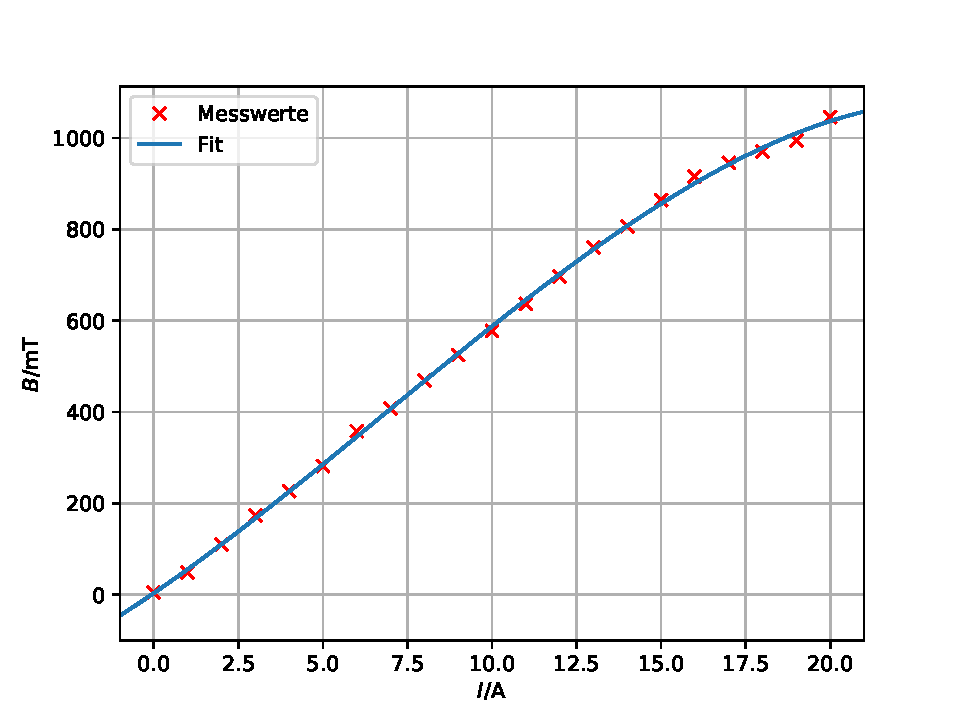
\includegraphics[width = \textwidth]{../Messdaten/plots/hysterese_aufsteigend.pdf}
  \caption{Aufsteigender Strom $I$.}
  \label{fig: hysterese_aufsteigend}
\end{subfigure}
\hfill
  \begin{subfigure}{0.48\textwidth}
  \centering
  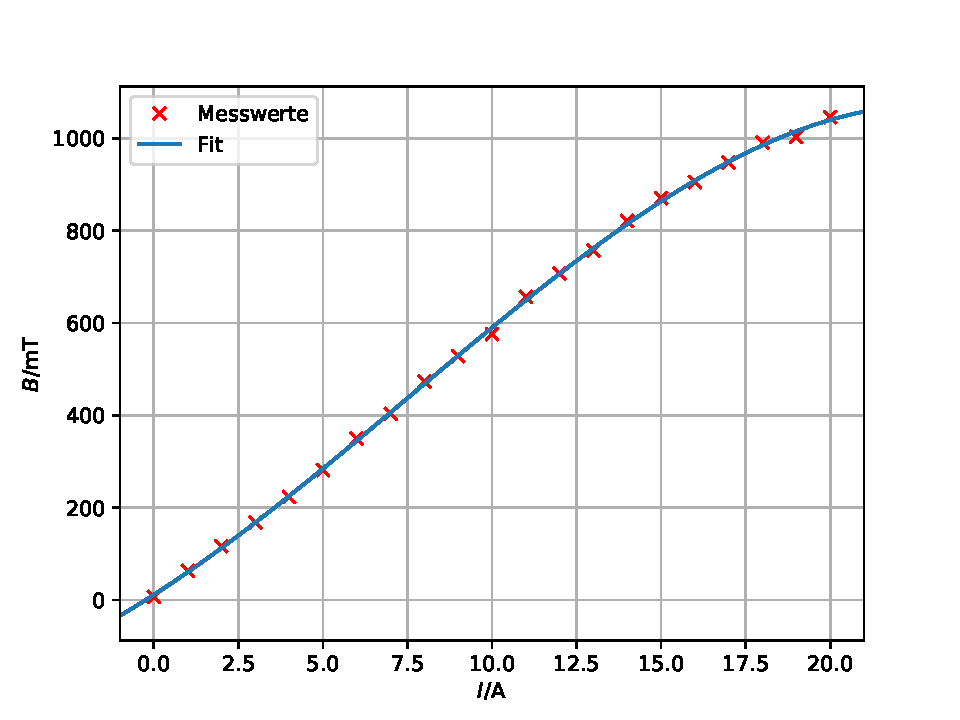
\includegraphics[width = \textwidth]{../Messdaten/plots/hysterese_absteigend.pdf}
  \caption{Absteigender Strom $I$.}
  \label{fig: hysterese_absteigend}
\end{subfigure}
\caption{Graphische Darstellung der Abhängigkeit $B(I)$ unter ab-/aufsteigendem Strom $I$ mit jeweiliger Regressionskurve.}
\label{fig: hysterese_fit}
\end{figure}
Im Folgenden wird Gleichung \eqref{eq: fitfuntion_hysterese} mit den Parametern \eqref{eq: params_up}
verwendet um den notwendigen Zusammenhang zwischen angelegtem Strom $I$ und magnetischer Flussdichte $B$ herzustellen.

\begin{figure}
  \centering
  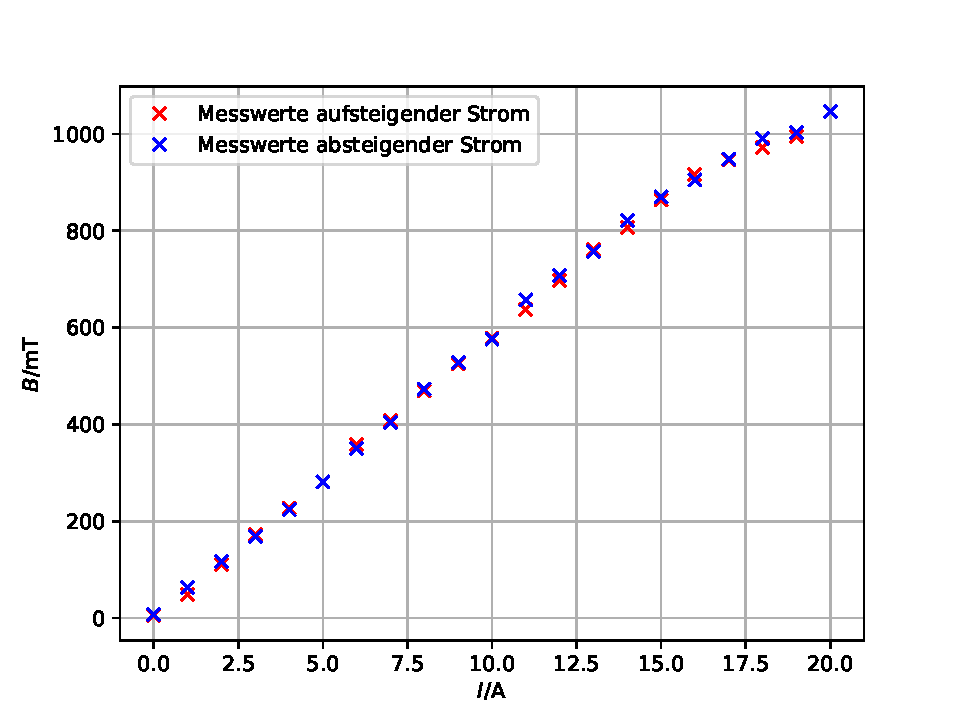
\includegraphics[width = \textwidth]{../Messdaten/plots/hysterese_data.pdf}
  \caption{Graphische Darstellung der Messwerte zur Bestimmung des Zusammenhangs $B(I)$ zwischen angelegtem Strom $I$ und
  magnetischer Flussdichte $B$ des Elektromagneten.}
  \label{fig: hysterese_gesamt}
\end{figure}
\begin{figure}
  \centering
  \begin{subfigure}{0.48\textwidth}
    \centering
  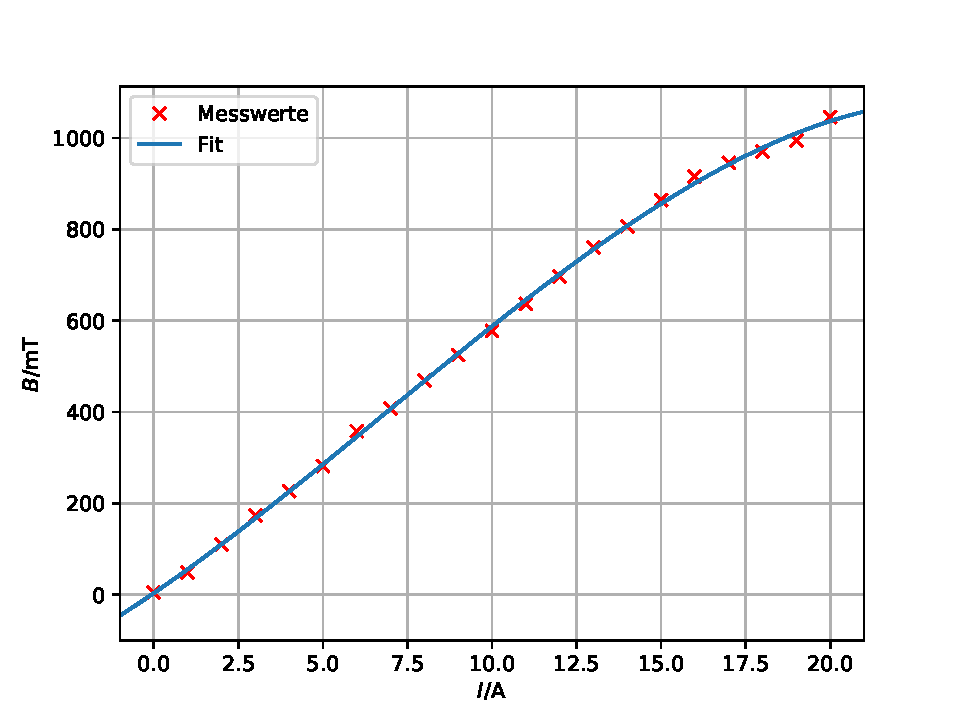
\includegraphics[width = \textwidth]{../Messdaten/plots/hysterese_aufsteigend.pdf}
  \caption{Aufsteigender Strom $I$.}
  \label{fig: hysterese_aufsteigend}
\end{subfigure}
\hfill
  \begin{subfigure}{0.48\textwidth}
  \centering
  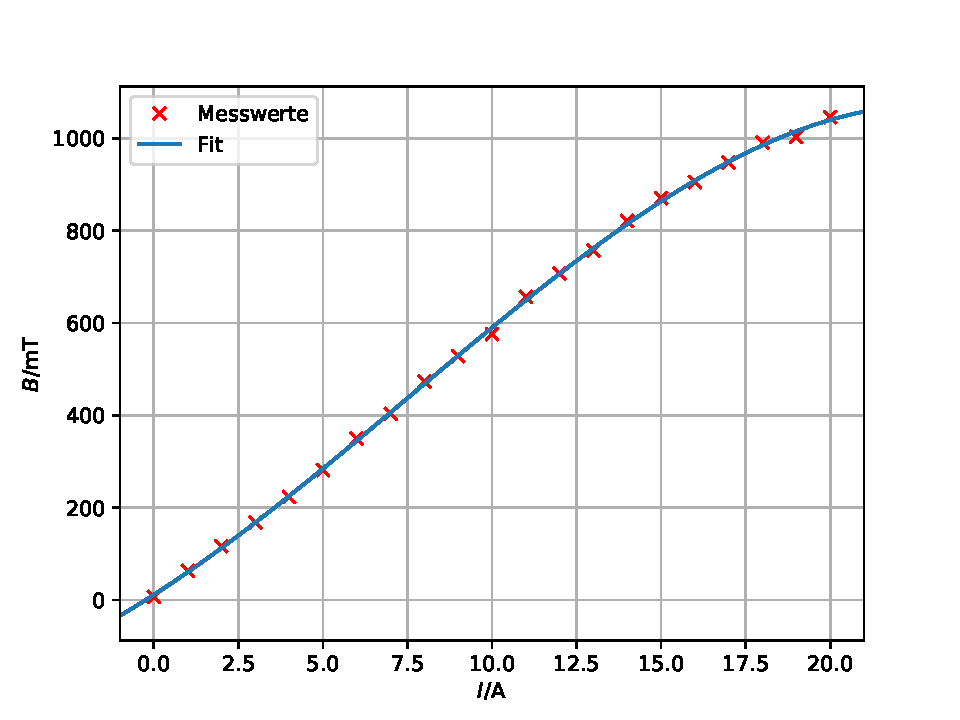
\includegraphics[width = \textwidth]{../Messdaten/plots/hysterese_absteigend.pdf}
  \caption{Absteigender Strom $I$.}
  \label{fig: hysterese_absteigend}
\end{subfigure}
\caption{Graphische Darstellung der Abhängigkeit $B(I)$ unter ab-/aufsteigendem Strom $I$ mit jeweiliger Regressionskurve.}
\label{fig: hysterese_fit}
\end{figure}
Im Folgenden wird Gleichung \eqref{eq: fitfuntion_hysterese} mit den Parametern \eqref{eq: params_up}
verwendet um den notwendigen Zusammenhang zwischen angelegtem Strom $I$ und magnetischer Flussdichte $B$ herzustellen.

\subsection{Analyse der roten $\sigma$-Linien}
Die Aufspaltung der roten Spektrallinie ist in Abbildung \ref{fig: aufspaltung_rot} dargestellt. Zur quantitativen Analyse der Auspaltung wird das
Resultat unter anliegendem Strom von $I = \SI{10}{\ampere}$ verwendet. Gemäß Formel \eqref{eq: fitfuntion_hysterese} bedingt dieser
eine magnetische Flussdichte von $B = \SI{587(3)}{\milli\tesla}$.
\begin{figure}
  \centering
  \includegraphics[width = 0.7\textwidth]{../Messdaten/bilder_v27/messung_1_rot_sigma/aufspaltung_rot.png}
  \caption{Aufgenommene Intensitätsstreifen des roten Lichtes unter (von oben nach unten) $\SI{0}{\ampere}$, $\SI{7.5}{\ampere}$ und $\SI{10}{\ampere}$.}
  \label{fig: aufspaltung_rot}
\end{figure}
Die Helligkeit in Abhängigkeit von der horizontalen Position auf den aufgenommenen Bilder ist in Abbildung \ref{fig: rot_intensität} für das unaufgespaltene
und aufgespaltene Beugungsbild dargestellt. Anhand dessen werden die Positionen von $12$ Intensitätsmaxima und ihrer Aufspaltungen
vermessen. Die Daten sind in Tabelle \ref{tab: peaks_rot} aufgeführt.
\begin{figure}
  \centering
  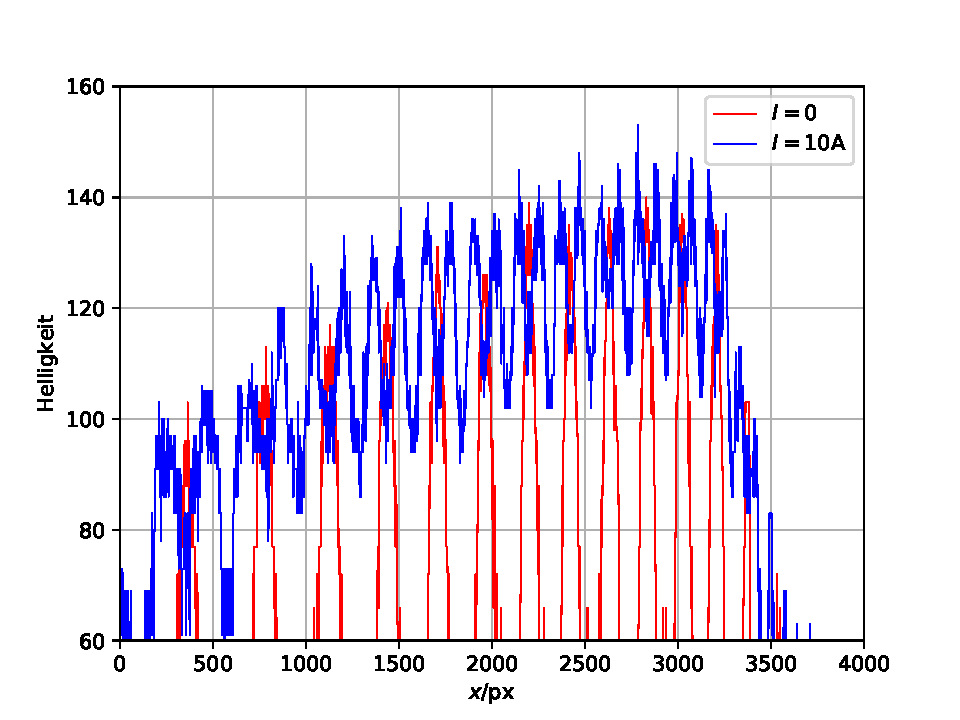
\includegraphics[width = 0.7\textwidth]{../Messdaten/plots/rot_sigma_intensitaet.pdf}
  \caption{Darstellung der Helligkeit der roten Linien in Abhängigkeit von der horizontalen Lage auf dem Foto.}
  \label{fig: rot_intensität}
\end{figure}
\begin{table}
\centering
\caption{Positionen $x_0$ und $x_{10}$ der Intensitätsmaxima unter $I= \SI{0}{\ampere}$ und $I= \SI{10}{\ampere}$.}
\label{tab: peaks_rot}
\begin{tabular}{S S[table-format=4.0] S[table-format=4.0] }
\toprule
{$x_0 /$ px} & \multicolumn{2}{c}{$x_{10} \:/\: $px} \\
\midrule
364 & 234 & 2145\\
784 & 470 & 2254\\
1132 & 693 & 2376\\
1436 & 865 & 2471\\
1705 & 1029 & 2579\\
1964 & 1207 & 2676\\
2201 & 1360 & 2782\\
2415 & 1511 & 2877\\
2632 & 1653 & 2980\\
2830 & 1775 & 3069\\
3022 & 1900 & 3166\\
3205 & 2017 & 3255\\
\bottomrule
\end{tabular}
\end{table}

Eine graphische Darstellung der abgelesenen Intensitätsmaxima befindet sich in den Abbildungen \ref{fig: peaks_rot_0} und \ref{fig: peaks_rot_10}.
\begin{figure}
  \centering
  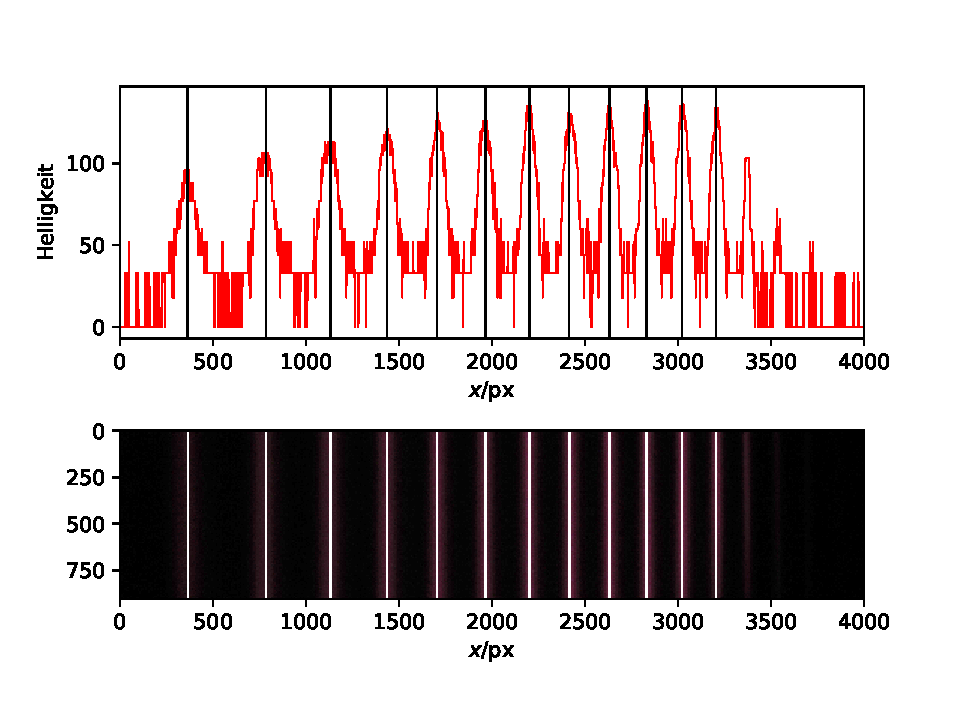
\includegraphics[width = 0.7\textwidth]{../Messdaten/plots/peaks_rot_sigma_0.pdf}
  \caption{Darstellung der abgelesenen Lagen der Intesitätsmaxima für das Beugungsbild unter $I =0$A.}
  \label{fig: peaks_rot_0}
\end{figure}
\begin{figure}
  \centering
  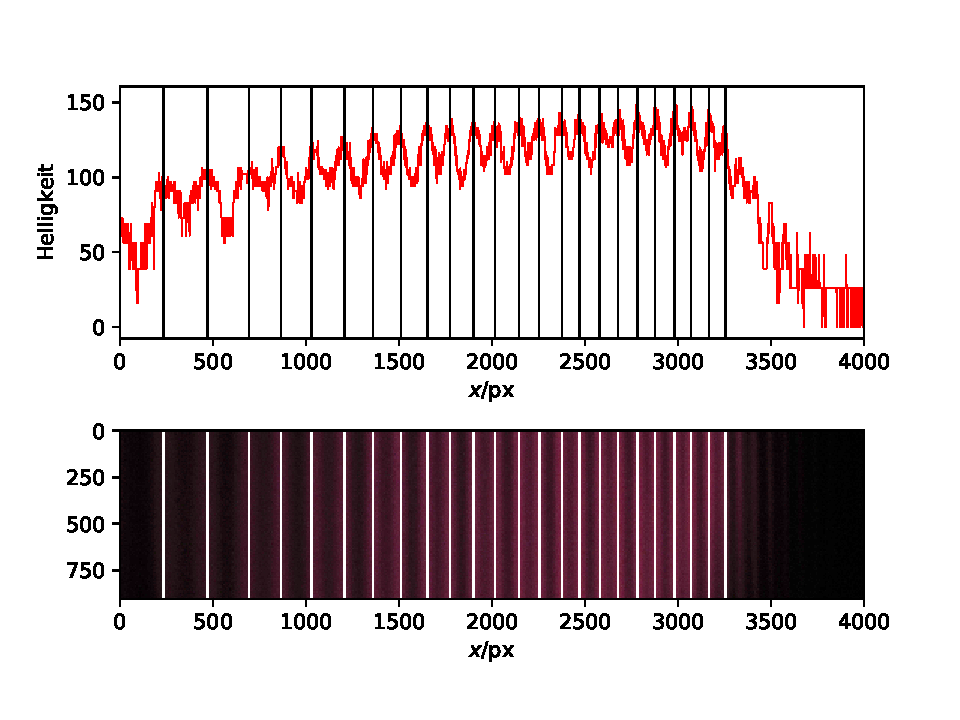
\includegraphics[width = 0.7\textwidth]{../Messdaten/plots/peaks_rot_sigma_10.pdf}
  \caption{Darstellung der abgelesenen Lagen der Intesitätsmaxima für das Beugungsbild unter $I =10$A.}
  \label{fig: peaks_rot_10}
\end{figure}
Die für die Berechnung der Wellenlängenänderung relevanten Abstände $\Delta s_i$ und $\delta s_i$ sind in Tabelle \ref{tab: abstände_rot}
aufgeführt. Mit Hilfe der Gleichungen \eqref{} berechnen sich hieraus die Wellenlängenaufspaltung $\Delta \lambda$, die
Energieaufspaltung $\Delta E$ und schließlich die Werte für die Übergangs-Lande-Faktoren $g$. Alle Ergebnisse sind ebenfalls in
Tabelle \ref{tab: abstände_rot} eingetragen. Als Mittelwert für den Lande-Faktor ergibt sich
\begin{equation}
  g = \num{1.045(5)}.
\end{equation}
\input{../Messdaten/tabs/abstände_rot.tex}
